% =====================================================================
%  Kleines Symbol des Shaper Origin (von vorn) für den Kopf der
%  Betriebsanweisung (\BAsetup{bildcode=...}). Ohne zeichnungen/stil.tex
%  lauffähig. Selbst gezeichnet.
% =====================================================================
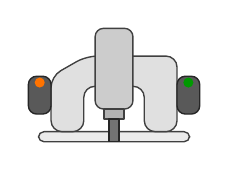
\begin{tikzpicture}[x=0.16mm, y=0.16mm, line width=0.5pt, line join=round]
  % Grundplatte
  \draw[fill=black!8, draw=black!75, rounded corners=2] (-60,0) rectangle (60,8);
  % Gehäuse mit Öffnung für die Spindel
  \draw[fill=black!12, draw=black!75, rounded corners=4] (-50,8) -- (-50,52) -- (-22,68)
    -- (50,68) -- (50,8) -- (24,8) -- (24,44) -- (-24,44) -- (-24,8) -- cycle;
  % Griffe mit Tasten
  \draw[fill=black!65, draw=black!85, rounded corners=3] (-68,22) rectangle (-50,52);
  \draw[fill=black!65, draw=black!85, rounded corners=3] (50,22) rectangle (68,52);
  \fill[orange!90!red] (-59,47) circle (4);
  \fill[green!60!black] (59,47) circle (4);
  % Spindel, Spannmutter, Fräser
  \draw[fill=black!20, draw=black!75, rounded corners=3] (-15,26) rectangle (15,90);
  \draw[fill=black!30, draw=black!75] (-8,18) rectangle (8,26);
  \draw[fill=black!55, draw=black!85] (-4,0) rectangle (4,18);
\end{tikzpicture}
